\documentclass{templateNote}
\usepackage{tcolorbox}
\usepackage{tabularx}
\usepackage{hyperref}
\usepackage{amsmath}
\usepackage{amssymb}
\usepackage{pdflscape}
\usepackage{tikz}
\usepackage{pdfpages}
\usepackage{soul}
\usepackage{media9}
\usepackage{adjustbox}
\usepackage{pdfpages}
% \usepackage[spanish,es-noquoting]{babel}

\begin{document}
\linklogoU{https://www.ubiobio.cl/w/}
\linklogoD{https://github.com/NicoGomezM}
\imagenlogoU{img/logo-ubb-txt-face.png}
\imagenlogoD{img/logoNGMFormal_sinF.png}
\titulo{Laboratorio 4: Display de 7 segmentos}
\asignatura{Laboratorio Arquitectura de Computadores}
\autor{
    Nicolás \textsc{Gómez Morgado}
}

\portada
\margenes

\section*{Ejercicios solicitados}

\begin{enumerate}
    \item Tabla completada \textbf{20 pts.}
    \begin{figure}[H]
        \centering
        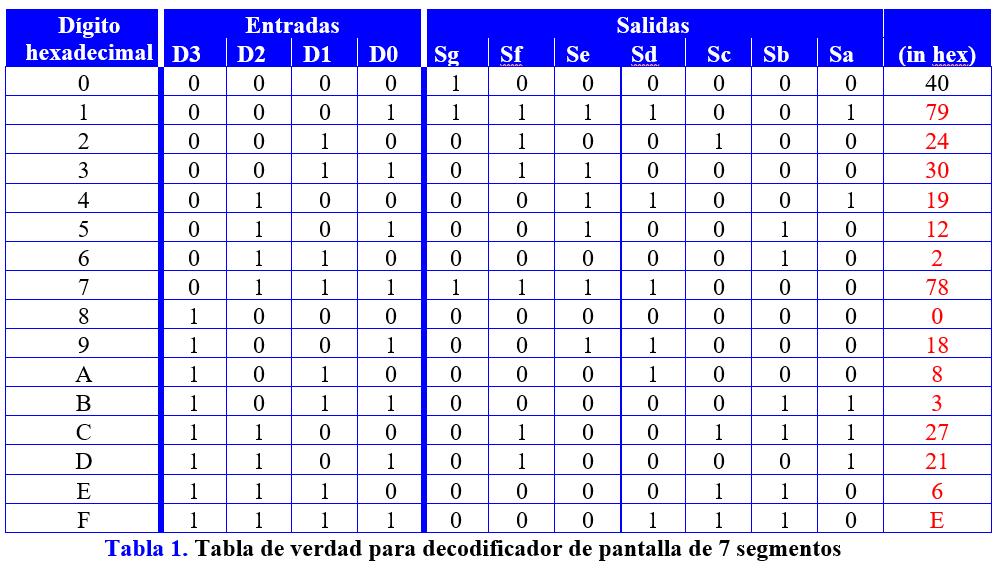
\includegraphics[width=0.8\textwidth]{img/tabla.png}
        \caption{Tabla de verdad}
        \label{fig:tabla}
    \end{figure}
    Para mejorar la comprension y la visualizacion de la tabla de verdad, he decidido modificar los valores de la tabla de verdad, siendo 1 para cuando el segmento se active y 0 para cuando no se active. Quedando de la siguiente manera:
    \begin{table}[H]
        \centering
        \begin{tabular}{|c|c|c|c|c|c|c|c|c|}
            \hline
            \textbf{Val} & \textbf{$S_g$} & \textbf{$S_f$} & \textbf{$S_e$} & \textbf{$S_d$} & \textbf{$S_c$} & \textbf{$S_b$} & \textbf{$S_a$} & \textbf{HEX} \\ \hline
            0            & 0              & 1              & 1              & 1              & 1              & 1              & 1              & 3F         \\ \hline
            1            & 0              & 0              & 0              & 0              & 1              & 1              & 0              & 6          \\ \hline
            2            & 1              & 0              & 1              & 1              & 0              & 1              & 1              & 5B         \\ \hline
            3            & 1              & 0              & 0              & 1              & 1              & 1              & 1              & 4F         \\ \hline
            4            & 1              & 1              & 0              & 0              & 1              & 1              & 0              & 66         \\ \hline
            5            & 1              & 1              & 0              & 1              & 1              & 0              & 1              & 6D         \\ \hline
            6            & 1              & 1              & 1              & 1              & 1              & 0              & 1              & 7D         \\ \hline
            7            & 0              & 0              & 0              & 0              & 1              & 1              & 1              & 7          \\ \hline
            8            & 1              & 1              & 1              & 1              & 1              & 1              & 1              & 7F         \\ \hline
            9            & 1              & 1              & 0              & 0              & 1              & 1              & 1              & 67         \\ \hline
            A            & 1              & 1              & 1              & 0              & 1              & 1              & 1              & 77         \\ \hline
            B            & 1              & 1              & 1              & 1              & 1              & 0              & 0              & 7C         \\ \hline
            C            & 1              & 0              & 1              & 1              & 0              & 0              & 0              & 58         \\ \hline
            D            & 1              & 0              & 1              & 1              & 1              & 1              & 0              & 5E         \\ \hline
            E            & 1              & 1              & 1              & 1              & 0              & 0              & 1              & 79         \\ \hline
            F            & 1              & 1              & 1              & 0              & 0              & 0              & 1              & 71         \\ \hline
        \end{tabular}
    \end{table}
    \item Tus ecuaciones de salida para cada uno de los 7 segmentos. \textbf{25pts} \\\\
    Para la construcción de un led de 7 segemntos con 4 entradas, siendo estas A, B, C y D, las ecuaciones relacionadas con la tabla de verdad son las siguientes:
    \begin{itemize}
        \item $S_a$ = $\overline{A} \cdot \overline{B} \cdot \overline{C} \cdot D + \overline{A} \cdot B \cdot C \cdot \overline{D} + A \cdot \overline{B} \cdot C \cdot D + A \cdot B \cdot \overline{C} \cdot \overline{D}$ \\
        \item $S_b$ = $\overline{A} \cdot B \cdot \overline{C} \cdot \overline{D} + A \cdot B \cdot \overline{C} \cdot D + A \cdot B \cdot C \cdot \overline{D}$ \\
        \item $S_c$ = $\overline{A} \cdot \overline{B} \cdot C \cdot \overline{D} + A \cdot B \cdot \overline{C} \cdot D + A \cdot B \cdot C \cdot \overline{D}$ \\
        \item $S_d$ = $\overline{A} \cdot B \cdot \overline{C} \cdot D + \overline{A} \cdot B \cdot C \cdot \overline{D} + A \cdot \overline{B} \cdot C \cdot D + A \cdot B \cdot \overline{C} \cdot \overline{D}$ \\
        \item $S_e$ = $\overline{A} \cdot \overline{B} \cdot C \cdot D + A \cdot B \cdot \overline{C} \cdot \overline{D}$ \\
        \item $S_f$ = $\overline{A} \cdot \overline{B} \cdot \overline{C} \cdot D + \overline{A} \cdot B \cdot C \cdot \overline{D} + A \cdot \overline{B} \cdot C \cdot D$ \\
        \item $S_g$ = $\overline{A} \cdot B \cdot \overline{C} \cdot \overline{D} + \overline{A} \cdot B \cdot C \cdot D + A \cdot B \cdot \overline{C} \cdot D$
    \end{itemize}
    \newpage
    \item Una imagen de su esquema de Quartus que muestre la lógica de su decodificador de pantalla de 7 segmentos (como en el Laboratorio 3, File→Export generalmente funciona bien). \textbf{25pts}
    \begin{figure}[H]
        \centering
        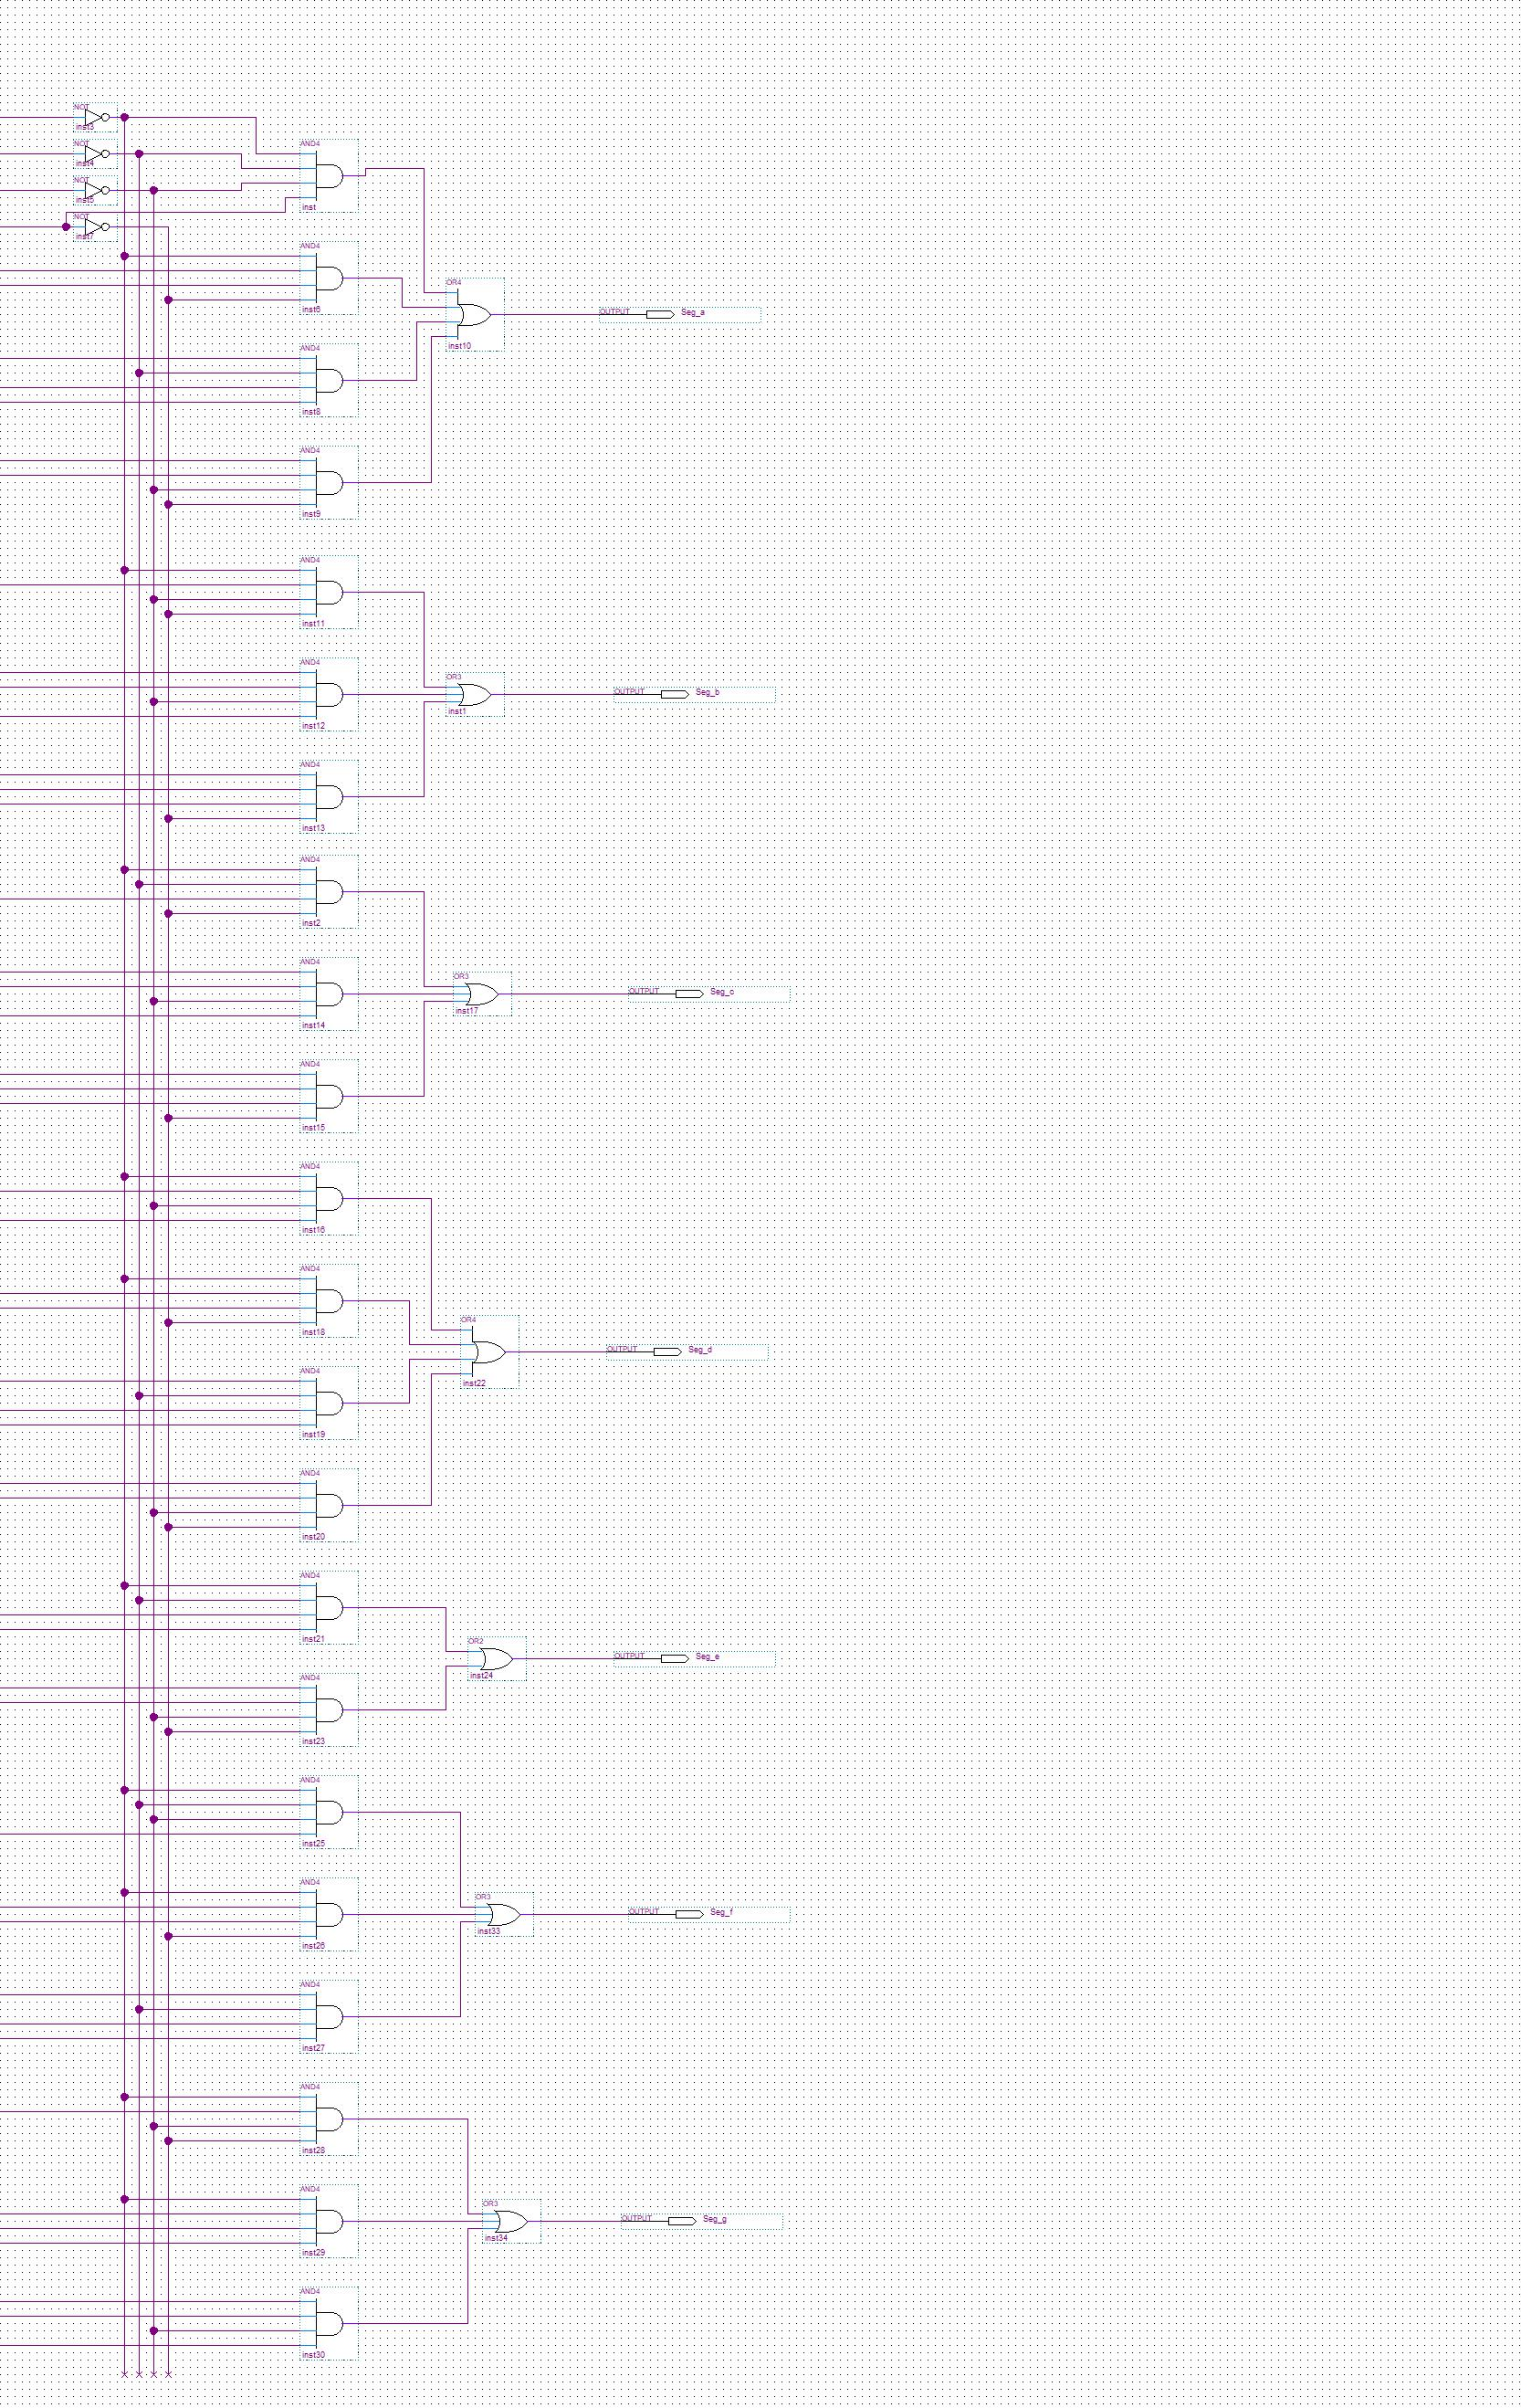
\includegraphics[width=0.8\textwidth]{img/7seg.jpg}
        \caption{Esquema de Quartus}
        \label{fig:esquema}
    \end{figure}
    % \begin{document}
    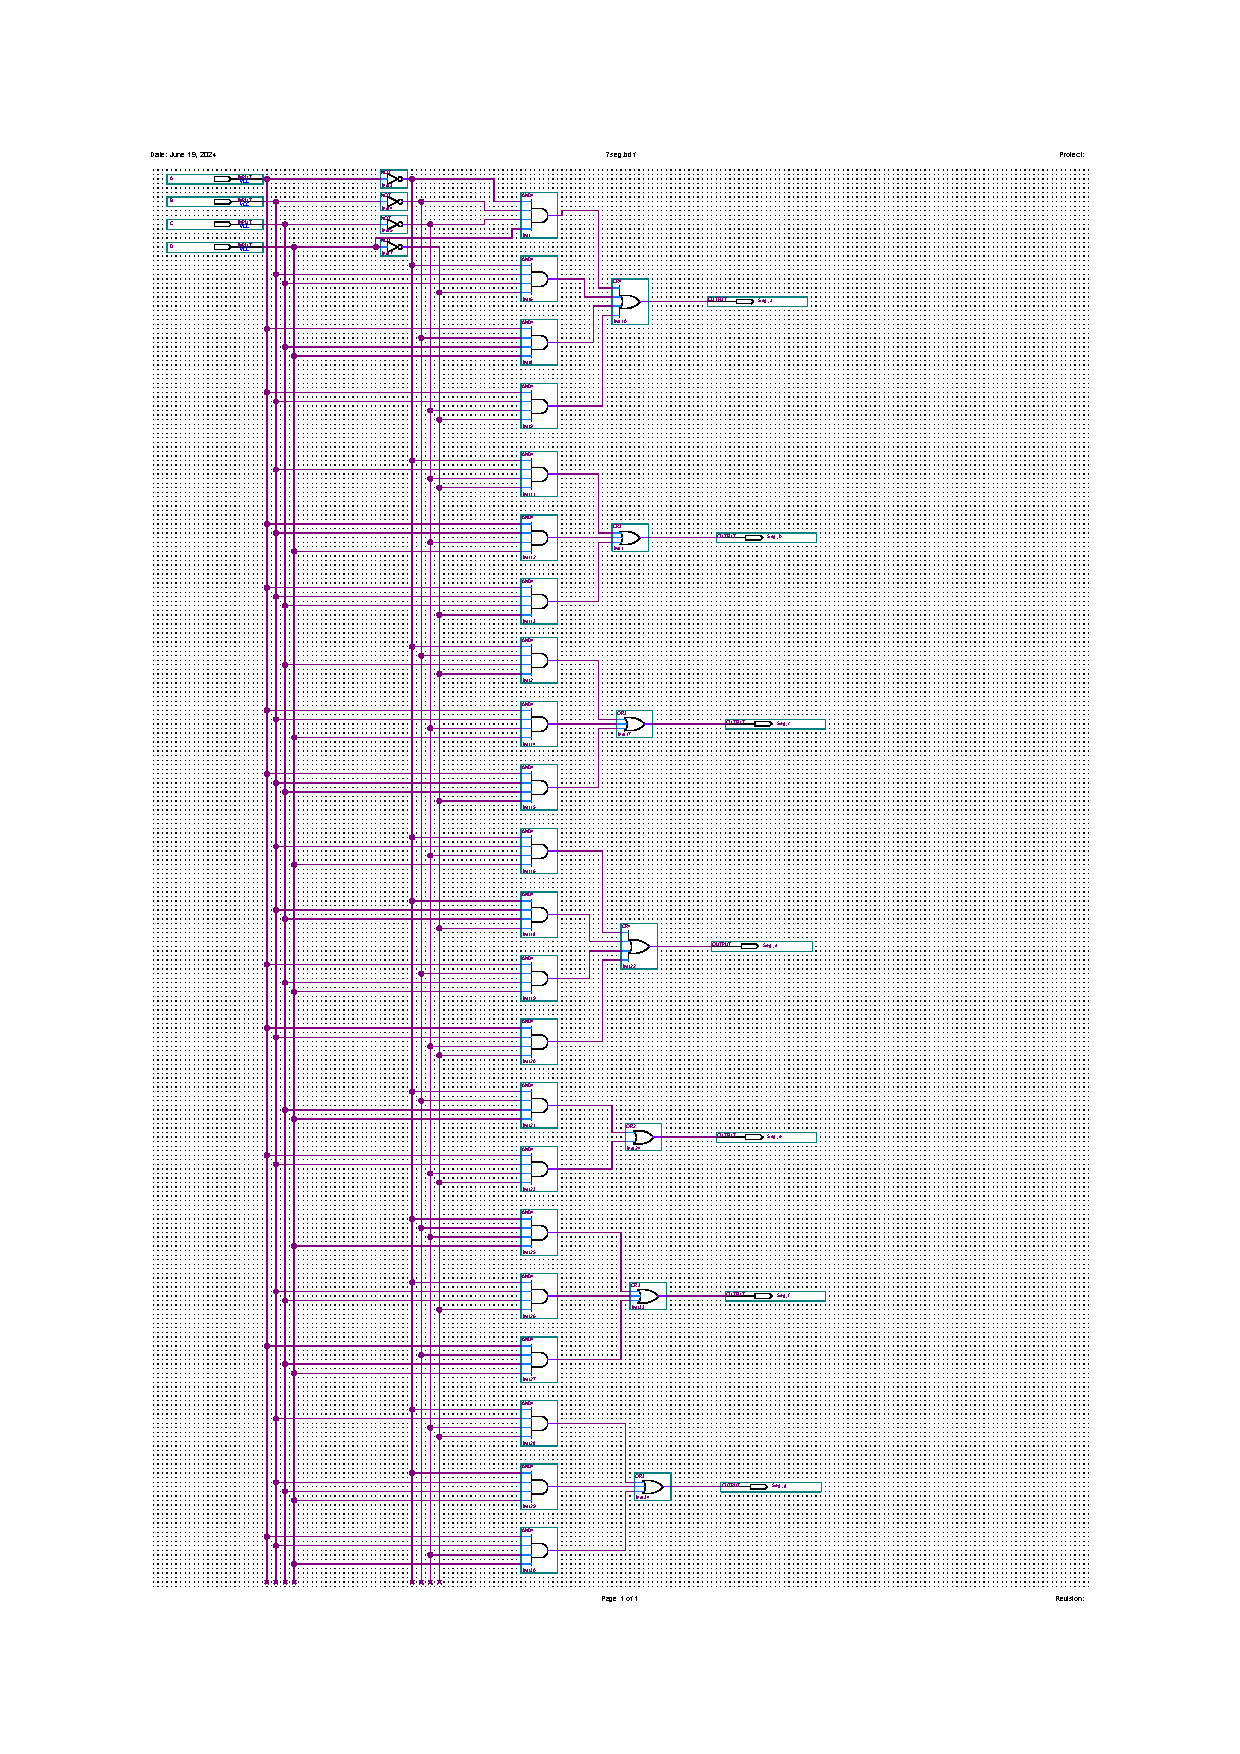
\includepdf[pages={1}]{7seg.pdf}
    % \end{document}
    \item Un párrafo que describa el método de diseño y la elección de diseño. \textbf{10pts} \\\\
    El método de diseño implementado se basa en facilitar la comprensión de la tabla de verdad. Para ello, se ha decidido modificar los valores de la tabla de verdad, asignando 1 cuando el segmento se activa y 0 cuando no se activa. Posteriormente, se obtuvieron las ecuaciones de salida para cada uno de los 7 segmentos, las cuales se implementaron en el software Quartus, con el fin de obtener el esquema de la lógica de decodificación de la pantalla de 7 segmentos. 
    \\Este diagrama se ha diseñado de manera que las conexiones sean fáciles de seguir visualmente, lo que facilita la comprensión de la lógica de decodificación de la pantalla de 7 segmentos.
    \item Una imagen de las formas de onda de simulación que muestra el funcionamiento correcto para todas las combinaciones de entrada a partir de 0 y llegar a F (Archivo → Exportar → Imagen...). Su forma de onda debe mostrar sus entradas en la parte superior y sus salidas en la parte inferior. Todos los valores deben mostrarse en hexadecimal para facilitar la lectura. \textbf{20pts}
    \begin{figure}[H]
        \centering
        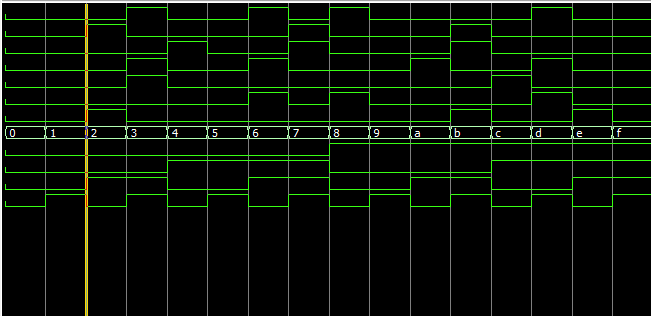
\includegraphics[width=0.8\textwidth]{img/ondas.png}
    \end{figure}
\end{enumerate}
\end{document}